\documentclass{beamer}
\usepackage[utf8]{inputenc}

\usepackage{array}
\usepackage{graphicx}
\usepackage{xcolor}
\usepackage{pgfplots}
\pgfplotsset{compat=1.13}
\usepackage{tikz}
\usetikzlibrary{arrows,arrows.meta,patterns,matrix,shapes,calc,positioning}
\usepackage{amsmath,amssymb,amsthm}

\usepackage{import}
\usepackage{catchfile}
\newcommand\loaddata[1]{\CatchFileDef\loadeddata{#1}{\endlinechar=-1}}

\newlength{\rs}

\definecolor{Rred}   {RGB}{191, 63, 63}%BF1F7F
\definecolor{Rgreen} {RGB}{ 63,191, 63}%1FBF1F
\definecolor{Rblue}  {RGB}{ 63, 63,255}%1F1FBF

\definecolor{Rpink}  {RGB}{255, 31,127}%FF1F7F
\definecolor{Rpurple}{RGB}{127, 31,255}%7F1FFF
\definecolor{Rorange}{RGB}{255,127, 31}%FF7F1F
\definecolor{Rlime}  {RGB}{127,255, 31}%7FFF1F
\definecolor{Rocean} {RGB}{ 31,127,255}%1F7FFF
\definecolor{Raqua}  {RGB}{ 31,255,127}%1FFF7F

\title{Neural Networks with Python and TensorFlow}
\author{Alexander J. Johnson}
\institute{Manchester Metropolitan University}
\date{2020}


\begin{document}

\frame{\titlepage}

\begin{frame}
    \frametitle{Aims and Objectives}

    \begin{itemize}
        \item Provide an introduction to a variety of neural network
            architectures.
        \item Implement the architectures in python using TensorFlow.
        \item Use neural networks to solve simple problems.
    \end{itemize}
\end{frame}

\begin{frame}
    \frametitle{Basis}

    Biological Neuron:
    \begin{center}
        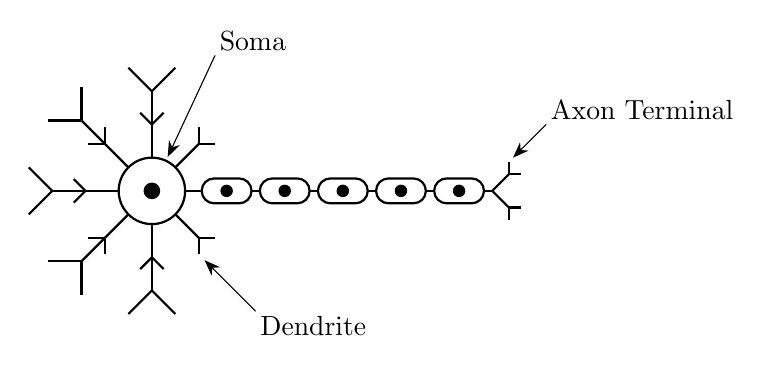
\begin{tikzpicture}%[x=1pt,y=1pt]
    [   > = {Stealth[scale=1.2]}
    ]
    \setlength{\rs}{1.5pt}
    % Nucleus
    \fill (0\rs,0\rs) circle (2\rs);
    % Soma
    \draw[thick] (0\rs,0\rs) circle (8\rs);
    % Dendrite
    \draw[thick] ( 45:8\rs) -- ( 45:16\rs);
        \draw[thick] ( 45:16\rs) -- ++(  0:4\rs);
        \draw[thick] ( 45:16\rs) -- ++( 90:4\rs);
    \draw[thick] ( 90:8\rs) -- ( 90:24\rs);
        \draw[thick] ( 90:16\rs) -- ++( 45:4\rs);
        \draw[thick] ( 90:16\rs) -- ++(135:4\rs);
        \draw[thick] ( 90:24\rs) -- ++( 45:8\rs);
        \draw[thick] ( 90:24\rs) -- ++(135:8\rs);
    \draw[thick] (135:8\rs) -- (135:24\rs);
        \draw[thick] (135:16\rs) -- ++( 90:4\rs);
        \draw[thick] (135:16\rs) -- ++(180:4\rs);
        \draw[thick] (135:24\rs) -- ++( 90:8\rs);
        \draw[thick] (135:24\rs) -- ++(180:8\rs);
    \draw[thick] (180:8\rs) -- (180:24\rs);
        \draw[thick] (180:16\rs) -- ++(135:4\rs);
        \draw[thick] (180:16\rs) -- ++(225:4\rs);
        \draw[thick] (180:24\rs) -- ++(135:8\rs);
        \draw[thick] (180:24\rs) -- ++(225:8\rs);
    \draw[thick] (225:8\rs) -- (225:24\rs);
        \draw[thick] (225:16\rs) -- ++(180:4\rs);
        \draw[thick] (225:16\rs) -- ++(270:4\rs);
        \draw[thick] (225:24\rs) -- ++(180:8\rs);
        \draw[thick] (225:24\rs) -- ++(270:8\rs);
    \draw[thick] (270:8\rs) -- (270:24\rs);
        \draw[thick] (270:16\rs) -- ++(225:4\rs);
        \draw[thick] (270:16\rs) -- ++(315:4\rs);
        \draw[thick] (270:24\rs) -- ++(225:8\rs);
        \draw[thick] (270:24\rs) -- ++(315:8\rs);
    \draw[thick] (315:8\rs) -- (315:16\rs);
        \draw[thick] (315:16\rs) -- ++(270:4\rs);
        \draw[thick] (315:16\rs) -- ++(360:4\rs);
    % Axon
    \draw[thick] (8\rs,0\rs) -- (12\rs,0\rs);
    \draw[thick,rounded corners=3\rs] (12\rs,-3\rs) rectangle (24\rs,3\rs);
        \fill (18\rs,0\rs) circle (1.5\rs);
    \draw[thick] (24\rs,0\rs) -- (26\rs,0\rs);
    \draw[thick,rounded corners=3\rs] (26\rs,-3\rs) rectangle (38\rs,3\rs);
        \fill (32\rs,0\rs) circle (1.5\rs);
    \draw[thick] (38\rs,0\rs) -- (40\rs,0\rs);
    \draw[thick,rounded corners=3\rs] (40\rs,-3\rs) rectangle (52\rs,3\rs);
        \fill (46\rs,0\rs) circle (1.5\rs);
    \draw[thick] (52\rs,0\rs) -- (54\rs,0\rs);
    \draw[thick,rounded corners=3\rs] (54\rs,-3\rs) rectangle (66\rs,3\rs);
        \fill (60\rs,0\rs) circle (1.5\rs);
    \draw[thick] (66\rs,0\rs) -- (68\rs,0\rs);
    \draw[thick,rounded corners=3\rs] (68\rs,-3\rs) rectangle (80\rs,3\rs);
        \fill (74\rs,0\rs) circle (1.5\rs);
    % Axon terminal
    \draw[thick] (80\rs,0\rs) -- (82\rs,0\rs);
        \draw[thick] (82\rs,0\rs) -- (86\rs,4\rs);
            \draw[thick] (86\rs,4\rs) -- (86\rs,7\rs);
            \draw[thick] (86\rs,4\rs) -- (89\rs,4\rs);
        \draw[thick] (82\rs,0\rs) -- (86\rs,-4\rs);
            \draw[thick] (86\rs,-4\rs) -- (86\rs,-7\rs);
            \draw[thick] (86\rs,-4\rs) -- (89\rs,-4\rs);
    % Labels
    % Soma
    \draw[<-] (65:9\rs) -- (65:36\rs);
    \node[anchor=south west,inner sep=1\rs] at (65:36\rs) {Soma};
    % Dendrite
    %\draw[latex'-] (225:25\rs) -- (225:36\rs);
    \draw[<-] (12.7\rs,-16.7\rs) -- (25\rs,-29\rs);
    \node[anchor=north west,inner sep=1\rs] at (25\rs,-29\rs) {Dendrite};
    % Axon Terminal
    \draw[<-] (87\rs,8\rs) -- (95\rs,16\rs);
    \node[anchor=south west,inner sep=1\rs] at (95\rs,16\rs) {Axon Terminal};
\end{tikzpicture}

    \end{center}
    Receives signals via dendrites and soma,
    applies threshold,
    outputs via axon terminal.
\end{frame}

\begin{frame}
    \frametitle{Perceptron}
    
    \begin{align*}
        A_i = \begin{cases}
            1, & \sum_j w_{i,j}x_j > \theta\\
            0, & \text{otherwise}
        \end{cases}
    \end{align*}

    Boolean output.

    Weights adjusted according to activation and response correctness.
\end{frame}

\begin{frame}
    \frametitle{Modern Neural Network}
    
    \begin{align*}
        y_i = \phi \left(b + \sum_j w_{i,j}x_j\right)
    \end{align*}

    Weights adjusted via backpropagation / chain rule.

    \begin{align*}
        w_i' = w_i + \eta\frac{\partial f}{\partial w_i}
    \end{align*}
\end{frame}

\begin{frame}
    \frametitle{Convolutional}
    
    Neurons only connect to regions of previous layers.
\end{frame}

\end{document}
